	\paragraph{QuizziPedia::Front-End::QuizziPediaServiceWorker}
		
		\label{QuizziPedia::Front-End::QuizziPediaServiceWorker}
		
		\begin{figure}[ht]
			\centering
			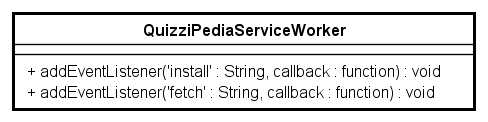
\includegraphics[scale=0.45,keepaspectratio]{UML/Classi/Front-End/QuizziPedia_Front-end_QuizziPediaServiceWorker.png}
			\caption{QuizziPedia::Front-End::QuizziPediaServiceWorker}
		\end{figure} \FloatBarrier
		
		\begin{itemize}

			\item \textbf{Descrizione}: un \textit{ServiceWorker\ped{G}} è uno script in esecuzione in background nel browser che non necessita necessariamente di avere ad esso collegato una pagina web e non necessita nemmeno l'iterazione con l'utente. La funzionalità principale dei \textit{ServiceWorker\ped{G}} è la capacità di intercettare e gestire le richieste di rete, tra cui anche gestire la cache di risposta. 
			Questo permette allo sviluppatore di gestire l'applicazione, dandone pieno controllo in ogni funzionalità, in modo che essa sia visualizzabile all'utente finale anche offline;
			\item \textbf{Utilizzo}: viene utilizzato per mostrare all'utente una pagina di errore dell'applicazione in caso in cui la rete non sia disponibile oppure nel caso in cui ci sia un malfunzionamento nel server ed esso non sia raggiungibile. La pagina mostrata non sarà perciò la classica pagina del browser di errore per problemi di rete ma una dell'applicazione in modo che l'esperienza dell'utente non venga diminuita;

			\item \textbf{Metodi}: 
			\begin{itemize}

				\item \texttt{+} \texttt{addEventListener('install': String, callback: function): void} \\ 
				Installa il \textit{ServiceWorker\ped{G}} tra i servizi disponibili del browser.
				\\
				\textbf{Parametri}:
				\begin{itemize}
					\item \texttt{'install': String}\\ Evento da collegare;
					\item \texttt{callback: function}\\ Funzione di callback che andrà a gestire l'evento.						
				\end{itemize}	
				\item \texttt{+} \texttt{addEventListener('fetch': String, callback: function): void} \\
				Gestisce il \textit{ServiceWorker\ped{G}} quando questo è già installato tra i servizi del browser.
				\\
				\textbf{Parametri}:
				\begin{itemize}
					\item \texttt{'fetch': String}\\ Evento da collegare;
					\item \texttt{callback: function}\\ Funzione di callback che andrà a gestire l'evento.						
				\end{itemize}	

							
			\end{itemize}
		\end{itemize}
		